\chapter{Convolutional neural networks}


\section{Convolutions}

\begin{description}
    \item[Convolution neuron] \marginnote{Convolution neuron}
        Neuron influenced by only a subset of neurons in the previous layer.
        
    \item[Receptive field] \marginnote{Receptive field}
        Dimension of the input image influencing a neuron.

    \item[Convolutional layer] \marginnote{Convolutional layer}
        Layer composed of convolutional neurons.
        Neurons in the same convolutional layer share the same weights and work as a convolutional filter.

        \begin{remark}
            The weights of the filters are learned.
        \end{remark}

        A convolutional layer has the following parameters:
        \begin{descriptionlist}
            \item[Kernel size] \marginnote{Kernel size}
                Dimension (i.e. width and height) of the filter.

            \item[Stride] \marginnote{Stride}
                Offset between each filter application (i.e. stride $>1$ reduces the size of the output image).

            \item[Padding] \marginnote{Padding}
                Artificial enlargement of the image.
                
                In practice, there are two modes of padding:
                \begin{descriptionlist}
                    \item[Valid] No padding applied.
                    \item[Same] Apply the minimum padding needed.
                \end{descriptionlist}

            \item[Depth] \marginnote{Depth}
                Number of different kernels to apply (i.e. augment the number of channels in the output image).
        \end{descriptionlist}

        The dimension along each axis of the output image is given by:
        \[ \frac{W + P - K}{S} + 1 \]
        where:
        \begin{itemize}
            \item $W$ is the size of the image (width or height).
            \item $P$ is the padding.
            \item $K$ is the kernel size.
            \item $S$ is the stride.
        \end{itemize}

        \begin{remark}
            If not specified, a kernel is applied to all the channels of the input image in parallel (but the weights of the kernel change at each channel).
        \end{remark}
\end{description}


\subsection{Parameters}

The number of parameters of a convolutional layer is given by:
\[ (K_\text{w} \cdot K_\text{h}) \cdot D_\text{in} \cdot D_\text{out} + D_\text{out} \]
where:
\begin{itemize}
    \item $K_\text{w}$ is the width of the kernel.
    \item $K_\text{h}$ is the height of the kernel.
    \item $D_\text{in}$ is the input depth.
    \item $D_\text{out}$ is the output depth.
\end{itemize}

Therefore, the number of FLOPS is of order:
\[ (K_\text{w} \cdot K_\text{h}) \cdot D_\text{in} \cdot D_\text{out} \cdot (O_\text{w} \cdot O_\text{h}) \]
where:
\begin{itemize}
    \item $O_\text{w}$ is the width of the output image.
    \item $O_\text{h}$ is the height of the output image.
\end{itemize}



\section{Backpropagation}

A convolution can be expressed as a dense layer by representing it through a sparse matrix.

Therefore, backpropagation can be executed in the standard way, 
with the only exception that the positions of the convolution matrix corresponding to 
the same cell of the kernel should be updated with the same value (e.g. the mean of all the corresponding updates).

\begin{example}
    Given a $4 \times 4$ image $I$ and a $3 \times 3$ kernel $K$ with stride $1$ and no padding:
    \[
        I = \begin{pmatrix} i_{0,0} & i_{0,1} & i_{0,2} & i_{0,3} \\ i_{1,0} & i_{1,1} & i_{1,2} & i_{1,3} \\ 
            i_{2,0} & i_{2,1} & i_{2,2} & i_{2,3} \\ i_{3,0} & i_{3,1} & i_{3,2} & i_{3,3} 
        \end{pmatrix} 
        \hspace{3em}
        K = \begin{pmatrix} w_{0,0} & w_{0,1} & w_{0,2} \\ w_{1,0} & w_{1,1} & w_{1,2} \\ w_{2,0} & w_{2,1} & w_{2,2} \end{pmatrix}
    \]
    The convolutional layer can be represented through a convolutional matrix and by flattening the image as follows:
    \[  
        \begin{pmatrix}
            w_{0,0} & 0         & 0         & 0         \\
            w_{0,1} & w_{0,0}   & 0         & 0         \\
            w_{0,2} & w_{0,1}   & 0         & 0         \\
            0       & w_{0,2}   & 0         & 0         \\
            w_{1,0} & 0         & w_{0,0}   & 0         \\
            w_{1,1} & w_{1,0}   & w_{0,1}   & w_{0,0}   \\
            w_{1,2} & w_{1,1}   & w_{0,2}   & w_{0,1}   \\
            0       & w_{1,2}   & 0         & w_{0,2}   \\
            w_{2,0} & 0         & w_{1,0}   & 0         \\
            w_{2,1} & w_{2,0}   & w_{1,1}   & w_{1,0}   \\
            w_{2,2} & w_{2,1}   & w_{1,2}   & w_{1,1}   \\
            0       & w_{2,2}   & 0         & w_{1,2}   \\
            0       & 0         & w_{2,0}   & 0         \\
            0       & 0         & w_{2,1}   & w_{2,0}   \\
            0       & 0         & w_{2,2}   & w_{2,1}   \\
            0       & 0         & 0         & w_{2,2}   \\
        \end{pmatrix}^T
        \cdot
        \begin{pmatrix} i_{0,0} \\ i_{0,1} \\ i_{0,2} \\ i_{0,3} \\ i_{1,0} \\ i_{1,1} \\ i_{1,2} \\ i_{1,3} \\ 
            i_{2,0} \\ i_{2,1} \\ i_{2,2} \\ i_{2,3} \\ i_{3,0} \\ i_{3,1} \\ i_{3,2} \\ i_{3,3} 
        \end{pmatrix} 
        =
        \begin{pmatrix} o_{0,0} \\ o_{0,1} \\ o_{1,0} \\ o_{1,1} \end{pmatrix} 
        \mapsto
        \begin{pmatrix} o_{0,0} & o_{0,1} \\ o_{1,0} & o_{1,1} \end{pmatrix} 
    \]
\end{example}



\section{Pooling layer}

\begin{description}
    \item[Pooling]
        Layer that applies a function as a filter.

        \begin{descriptionlist}
            \item[Max-pooling] \marginnote{Max-pooling}
                Filter that computes the maximum of the pixels within the kernel.

            \item[Mean-pooling] \marginnote{Mean-pooling}
                Filter that computes the average of the pixels within the kernel.
        \end{descriptionlist}
\end{description}



\section{Inception hypothesis}

\begin{description}
    \item[Depth-wise separable convolution] \marginnote{Depth-wise separable convolution}
        Decompose a 3D kernel into a 2D kernel followed by a 1D kernel.

        Given an input image with $C_\text{in}$ channels, 
        a single pass of a traditional 3D convolution uses a kernel of shape $k \times k \times C_\text{in}$
        to obtain an output of $1$ channel. 
        This is repeated for a desired $C_\text{out}$ number of times (with different kernels).
        \begin{figure}[H]
            \centering
            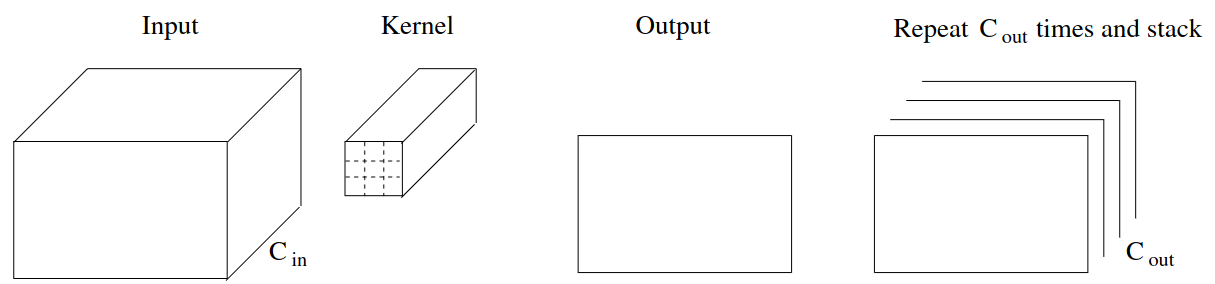
\includegraphics[width=0.65\linewidth]{./img/traditional_convolution.png}
            \caption{Example of traditional convolution}
        \end{figure}

        A single pass of a depth-wise separable convolution uses $C_\text{in}$ different $k \times k \times 1$ kernels first to obtain $C_\text{in}$ images.
        Then, a $1 \times 1 \times C_\text{in}$ kernel is used to obtain an output image of $1$ channel. 
        The last 1D kernel is repeated for a $C_\text{out}$ number of times (with different kernels).
        \begin{figure}[H]
            \centering
            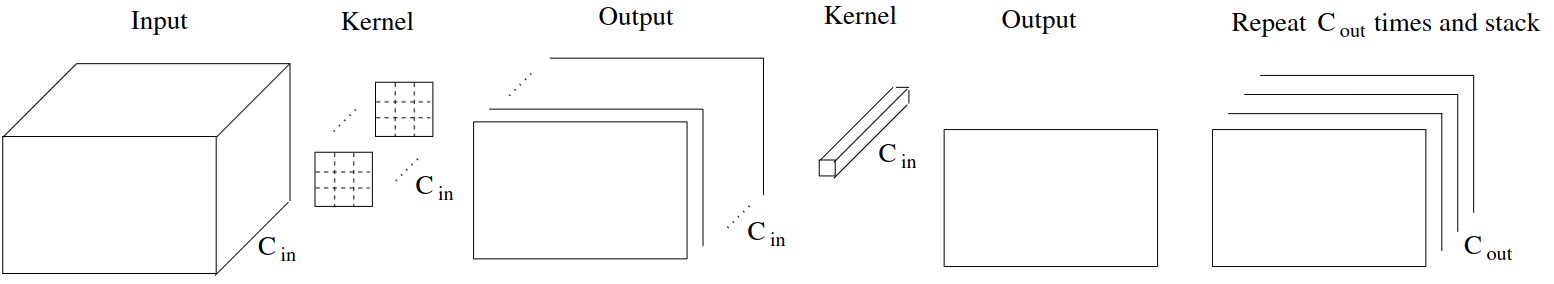
\includegraphics[width=0.85\linewidth]{./img/depthwise_separable_convolution.png}
            \caption{Example of depth-wise separable convolution}
        \end{figure}
\end{description}


\subsection{Parameters}

The number of parameters of a depth-wise separable convolutional layer is given by:
\[ (K_\text{w} \cdot K_\text{h}) \cdot D_\text{in} + (1 \cdot 1 \cdot D_\text{in}) \cdot D_\text{out} \]
where:
\begin{itemize}
    \item $K_\text{w}$ is the width of the kernel.
    \item $K_\text{h}$ is the height of the kernel.
    \item $D_\text{in}$ is the input depth.
    \item $D_\text{out}$ is the output depth.
\end{itemize}



\section{Residual learning}

\begin{description}
    \item[Residual connection] \marginnote{Residual connection}
        Sum the input of a layer to its output.
        \begin{figure}[H]
            \centering
            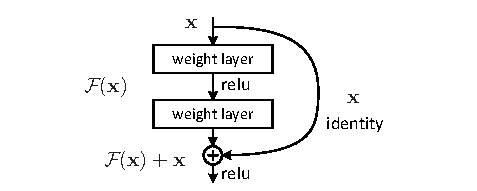
\includegraphics[width=0.5\linewidth]{./img/_residual_connection.pdf}
            \caption{Residual connection}
        \end{figure}

        \begin{remark}
            The sum operation can be substituted with the concatenation.
        \end{remark}

        \begin{remark}
            The effectiveness of residual connections is only shown empirically.
        \end{remark}

        \begin{remark}
            By adding the input, without passing through the activation function,
            might help to propagate the gradient from higher layers to lower layers
            and avoid the risk of vanishing gradient.
            
            Another interpretation is that, by learning the function $F(x) + x$, it is easier for the model to represent, if it needs to, the identity function as 
            the problem is reduced to learn $F(x) = 0$.
            On the other hand, without a residual connection, learning $F(x) = x$ from scratch might be harder.
        \end{remark}
\end{description}



\section{Transfer learning and fine-tuning}

\begin{description}
    \item[Transfer learning] \marginnote{Transfer learning}
        Reuse an existing model by appending some new layers to it.
        Only the new layers are trained.

    \item[Fine-tuning] \marginnote{Fine-tuning}
        Reuse an existing model by appending some new layers to it.
        The existing model (or part of it) is trained alongside the new layers.
\end{description}

\begin{remark}
    In computer vision, reusing an existing model makes sense as 
    the first convolutional layers tend to learn primitive concepts that are independent of the downstream task.
\end{remark}



\section{Other convolution types}

\begin{description}
    \item[Transposed convolution / Deconvolution] \marginnote{Transposed convolution / Deconvolution}
        Convolution to upsample the input (i.e. each pixel is upsampled into a $k \times k$ patch).

        \begin{remark}
            A transposed convolution can be interpreted as a normal convolution with stride $< 1$.
        \end{remark}


    \item[Dilated convolution] \marginnote{Dilated convolution}
        Convolution computed using a kernel that does not consider contiguous pixels.

        \begin{figure}[H]
            \centering
            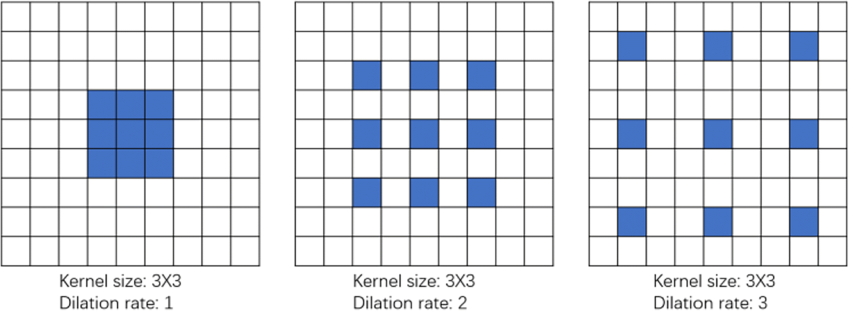
\includegraphics[width=0.5\linewidth]{./img/dilated_convolution.png}
            \caption{Examples of dilated convolutions}
        \end{figure}

        \begin{remark}
            Dilated convolutions allow the enlargement of the receptive field without an excessive number of parameters.
        \end{remark}

        \begin{remark}
            Dilated convolutions are useful in the first layers when processing high-resolution images (e.g. temporal convolutional networks).
        \end{remark}
\end{description}




\section{Normalization layer}

A normalization layer has the empirical effects of:
\begin{itemize}
    \item Stabilizing and possibly speeding up the training phase.
    \item Increasing the independence of each layer (i.e. maintain a similar magnitude of the weights at each layer).
\end{itemize}

\begin{description}
    \item[Batch normalization] \marginnote{Batch normalization}
        Given an input batch $X$, a batch normalization layer outputs the following:
        \[ \gamma \frac{X - \mu}{\sqrt{\sigma^2 + \varepsilon}} + \beta \]
        where:
        \begin{itemize}
            \item $\gamma$ and $\beta$ are learned parameters.
            \item $\varepsilon$ is a small constant.
            \item $\mu$ is the mean and $\sigma^2$ is the variance.
                Depending on when the layer is applied, these values change:
                \begin{descriptionlist}
                    \item[Training]
                        $\mu$ and $\sigma^2$ are computed from the input batch $X$.
        
                    \item[Inference] 
                        $\mu$ and $\sigma^2$ are computed from the training data. 
                        Usually, it is obtained as the moving average of the values computed from the batches during training.
                \end{descriptionlist}
        \end{itemize}

\end{description}